\chapter{Statistics of Radioactive Decays}


\section{Introduction}

In this lab, you will use a Geiger Counter to study the statistics of radioactive decays.


\section{Precautions}

\noindent
{\bf Precautions with the Geiger counter:}
\begin{itemize}
\item Leave the cable from the Geiger counter controller to the Geiger counter in place {\em at all times}.  This carries voltages of approximately 1000 volts.  If you leave the cable in place, nothing can be inadvertently plugged in (including fingers!)
\item Leave the Geiger tube in its holder.  It has a thin front window which is easily broken.
\end{itemize}

\noindent
{\bf Precautions with the radioactive source:}
\begin{itemize}
\item Don't touch the source.
\item Leave the source in the tray at all times.  The TA will provide the sources and handle moving them from place to place.
\item Radiation falls off as $1/r^2$.  So minimize your time near sources and maximize your distance from them.
\end{itemize}


\section{The Geiger Counter}

\begin{figure}[htbp]
\begin{center}
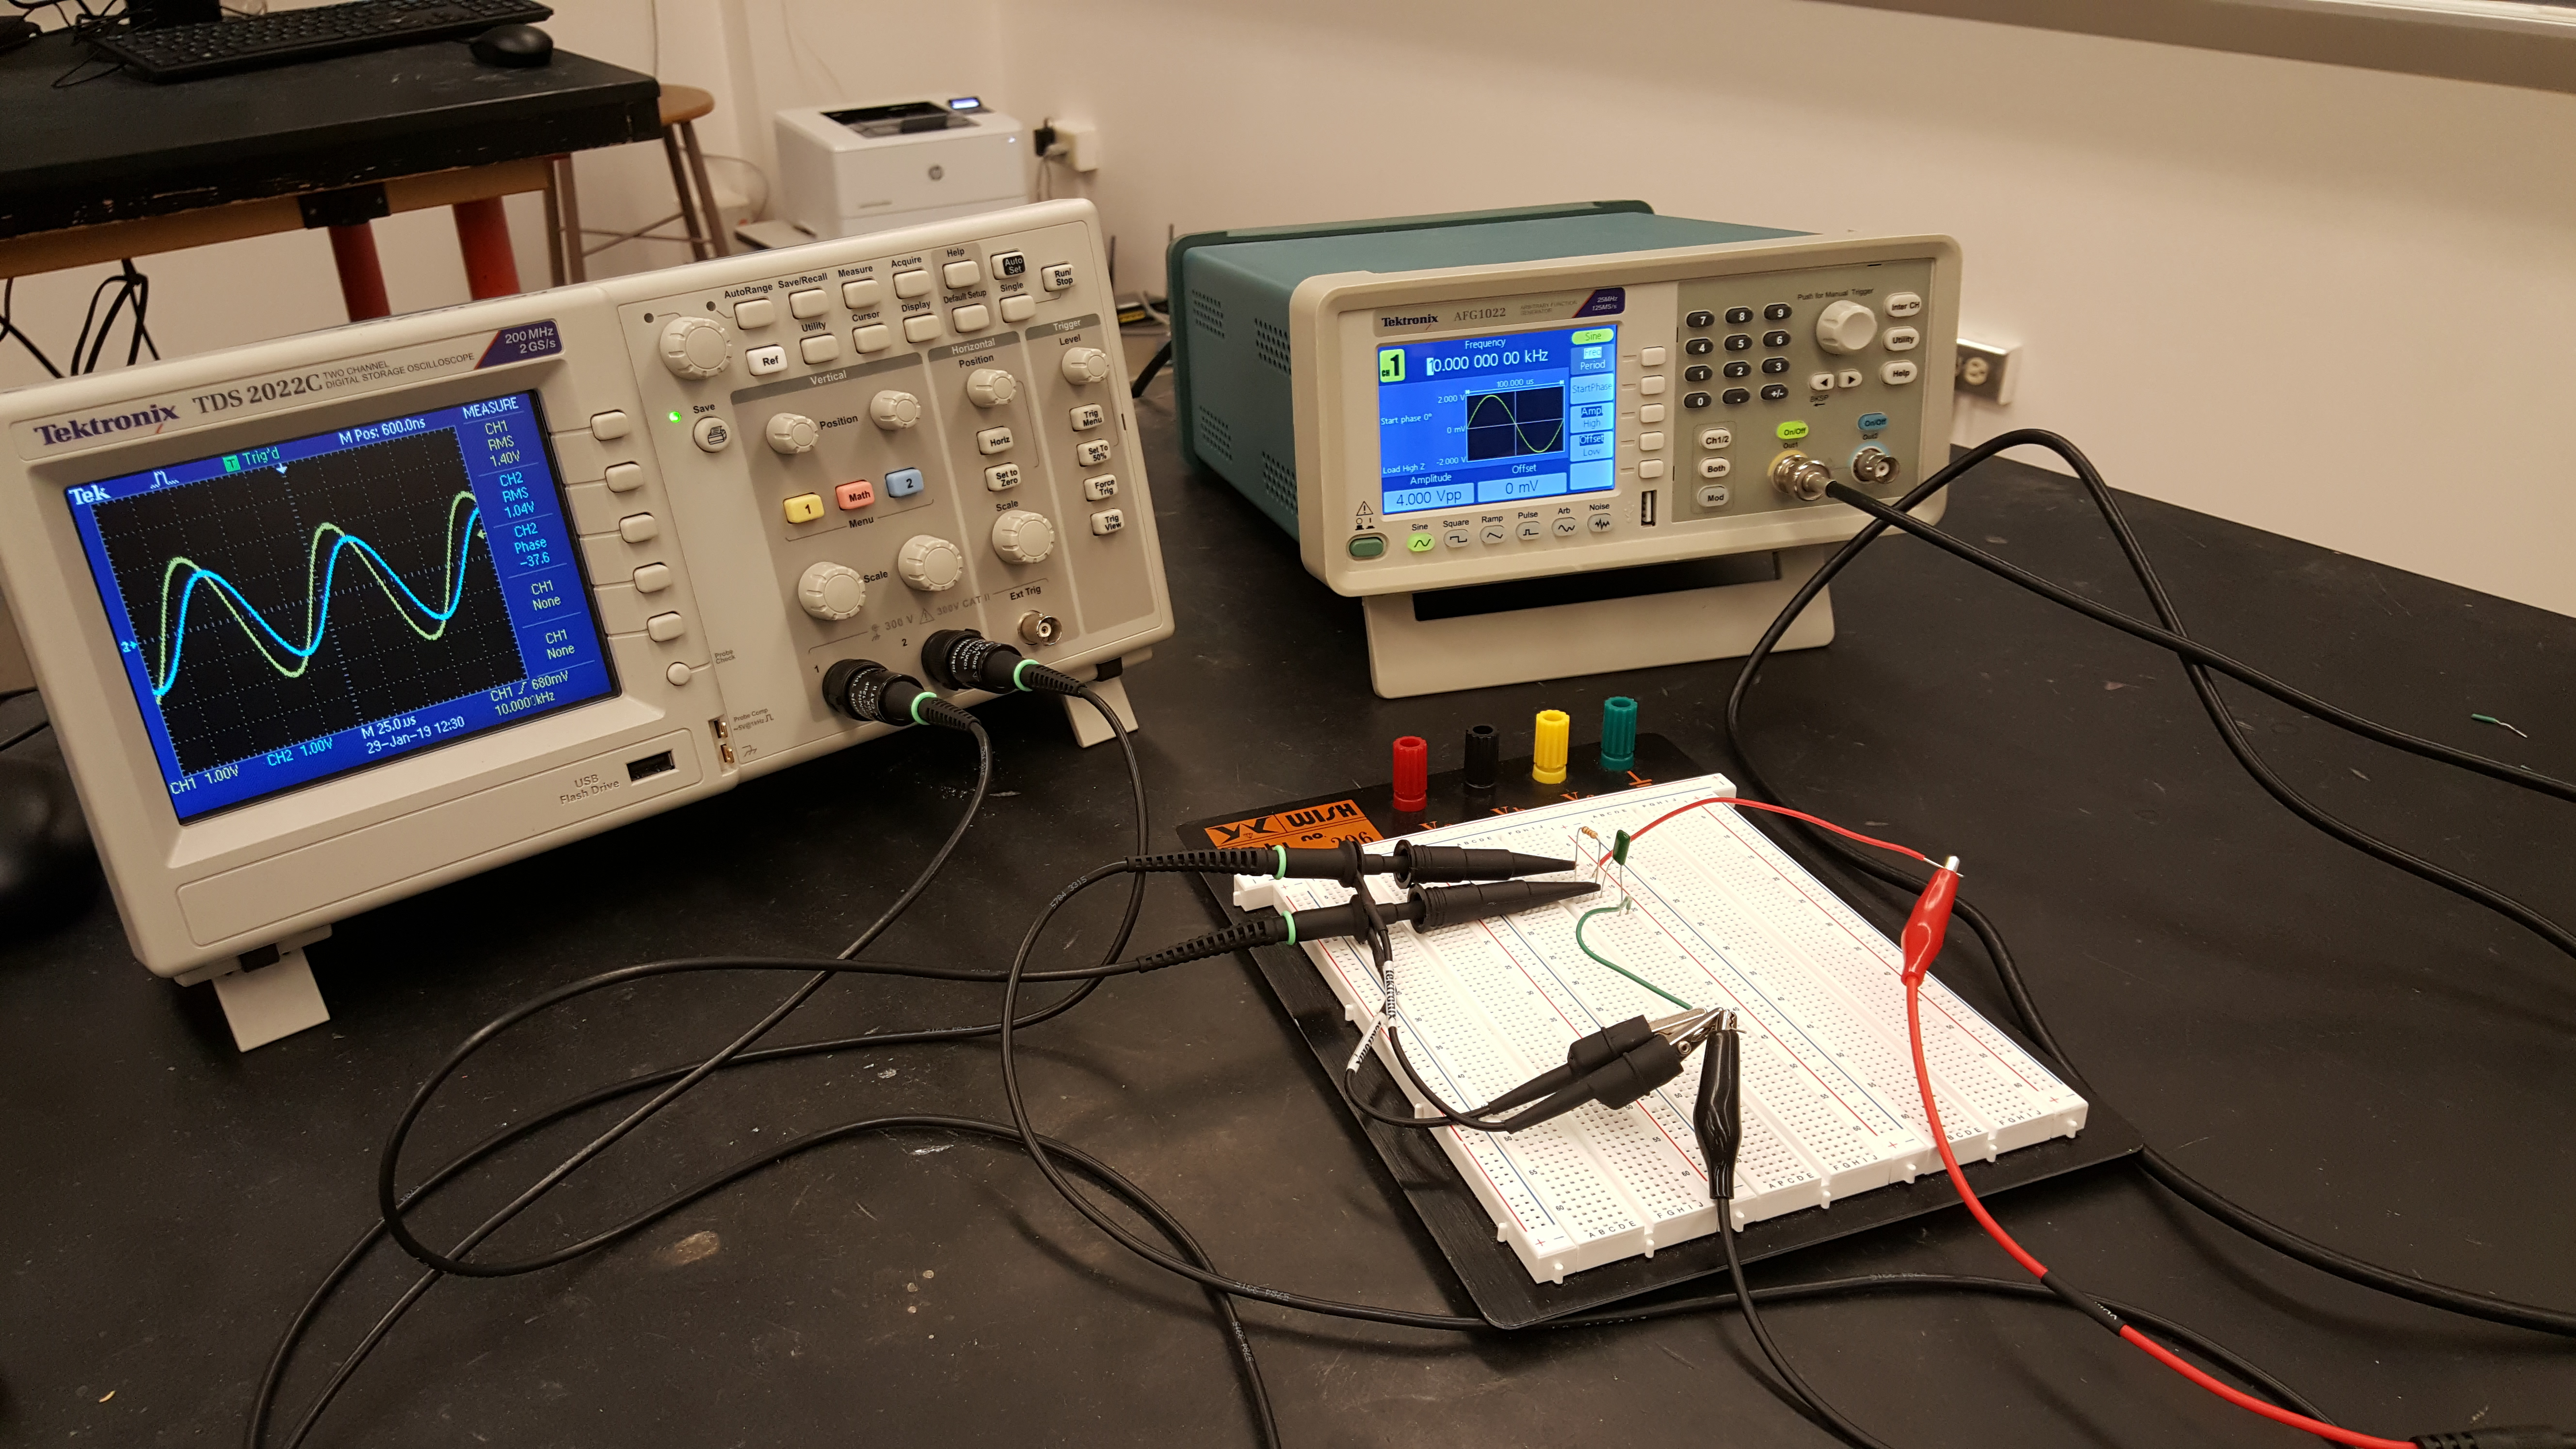
\includegraphics[height=0.22\textheight]{figs/labs/filters/filter_setup.jpg}
\end{center}
\caption{\label{fig:geiger_setup} The Geiger Counter assembly.}
\end{figure}

You lab bench will be prepared with a Geiger Counter assembly as shown in Fig.~ref

On the Geiger Controller, start with the HV set to zero at both the analog knob and the HV on-off switch.   Turn on the device and set the mode to``Test''.  In this mode, the counter will be incremented at a fixed rate of $60~\rm Hz$.   While in this mode, play around with the ``Count'', ``Reset'', and ``Lab-Chron'' analog timer reset dial until you understand how all of these features work.


\section{High-Voltage Calibration}

Next check that you have a source in the lowest drawer of the Geiger Counter holder, asking the TA for help if this is not the case.  Switch the mode back to ``Use'', which will now use the Geiger counter as input to the count.  With the HV still off, place the controller in ``Count'' mode, and verify that the rate, with no HV, is zero.  Now, with the controller still in ``Count'' mode, turn on the HV and turn the dial until you first see the counter incrementing.  Turn up the voltage to the next interval of 50 volts (e.g. if it first starts incrementing at 730 volts, set the dial to 750 volts).

Tabulate the number of counts in a 10 seconds interval, twice for each voltage level, in 50 volt steps from your starting voltage up to 1000 volts.  Do not exceed 1000 volts.  From the data, select the start of the plateau region, where increasing the voltage by 50 volts raises the rate by less than $10\%$.  With another measurement, confirm that the rate at this plateau is of order $100~\rm Hz$ (this will vary from source to source).

Look at the ``SCOPE'' output of the Geiger counter controller on your oscilloscope, with AC coupling, and verify that you see output pulses similar to those in Fig.~\ref{fig:geigerpulse}.



\section{Data Collection}

Ask the TA to place two layers of cardboard over your source.  

The rate should should be approximately 2~\rm Hz.

Measure counts for 100 trials each 2 seconds long.

When taking data, it's counter productive to reset the timer each
time.  Instead, simply stop the acquisition every N seconds, without
resetting the timer, e.g.: 2.1, 4.1,6.2,8.1,...  Note that the time
required to flip the switch introduces a slight offset, but this is
mostly ignored.








\section{Analysis}

Plot the measured gain as a function of frequency for your high-pass
and low-pass filter, and compare to the expected response.  Plot the
measured phase shift as a function of frequency for your high-pass and
low-pass filter, and compare to the expected response.
